\chapter{Technology Review}
\section{Overview}
This chapter looks at some of the technologies used throughout the project with a focus on why we choose them along with the benefits they possess. Also, covered is some of the technology researched and reviewed which was not used but lead us to our final implementation. We initially began with a number of questions that needed answering, which helped up with our research. 

\begin{itemize}
    \item What 3D Engine to use?
    \item What Speech Service?
    \item What technology to create a chat-bot?
    \item What Back-end?
\end{itemize}

\section{Application}
We knew we would need some form of gaming engine for the application itself. This would be the part of the project that the user would actually interact with. There are number of free gaming engines that we could have used however, we chose the Unity Engine as it is very well documented and powerful enough for our needs \cite{unity}.

\subsection{Unity}
This is the part of the application is where the user interacts with. After briefly looking at other game engines we chose unity it for below reasons:

\begin{itemize}
  \item Unity uses C\#. The reason this is good is because C\# is very versatile and supports many different programming styles \cite{csharp}. It can be used to created objects, make network requests and it is also Unity's default scripting language.
  \item It was apparent that 3D models and animations would be key to improving the experience of the application. Unity allowed us to add 3D models with ease. Unity also has a built in animator that allows you to animate these models by key-framing them and moving them as desired. All of this was very important to create a realistic training experience for the user.
  \item Another aspect that was important was to be able to connect to our back-end Flask server. Unity has built-in HTTP support allowing us to send necessary JSON data from the Speech-to-Text service to the server to be processed and a response sent back. \cite{unitywebrequest}.
  \item As mentioned Speech-to-Text (STT) and Text-to-Speech (TTS) is another important feature that was needed to enhance the realism for the user. After some research we found out that a lot of the STT and TTS services support Unity and supply their own packages for the engine, giving us options for when we decided on which STT and TTS service we were going to choose.
\end{itemize}

\section{HTTP}
HTTP or HyperText Transfer Protocol, is a protocol used by the world wide web to send messages from a client to a server or vice verse. It also defines how these messages are structured to inform the server or web browser what actions to take upon receiving a request \cite{rescorla2000http}. The reason we chose this approach is because for one, Unity has libraries that handle incoming and outgoing HTTP requests. Also, Flask uses HTTP making it very easy to communicate with our back-end server.

\section{JSON}
JavaScript Object Notation (JSON) is a widely used data interchange format for sending human readable messages across a network. It consists of attribute value pairs and array types which can be seen below in this simple example describing a person \cite{chen2014javascript}. We will use JSON to send all our web requests between our application and web server.

\begin{lstlisting}[language=JSON]
{
  "firstName": "John",
  "lastName": "Smith",
  "age": 27,
  "address": {
    "streetAddress": "21 2nd Street",
    "city": "New York",
    "state": "NY"
  },
  "phoneNumbers": [
    {
      "type": "home",
      "number": "212 555-1234"
    },
    {
      "type": "office",
      "number": "646 555-4567"
    }
  ],
  "children": [],
  "spouse": null
}
\end{lstlisting}

\section{Virtual Reality (VR)}
As one of the main goals outlined in the project was to create an immersive training experience for the end user, we felt we just couldn't get that level required from a conventional screen and controls. With this in mind we researched new technologies and deciding on using Virtual Reality (VR) to achieve this. VR can be sometimes mixed up with Augmented reality (AR). AR involves displaying virtual objects in a real-world environment, usually displayed on a mobile phone display through a camera. This had been implemented in some training experiences we looked at but wouldn't have met our initial goals or scenarios provided. However, a VR environment consists of a virtual three-dimensional (3D) space that a user can interact with objects and move around. \cite{isdale1998virtual}. This 3D space is encapsulated in a head-mounted display (HMD) or headset that the user can wear. Inside the headset, the user can become immersed and feel they are experiencing the real or the next best thing which was exactly what we required. \cite{isdale1998virtual}. 

\subsection{Google Cardboard}
Even though VR seemed like the solution for our immersive experience we still wanted to test it to ensure it was worth the time and investment. A solution to this was Google Cardboard (GC). GC is an affordable, simple to use cardboard frame that holds your smartphone device \cite{12335197120170501}. The user then holds the cardboard headset up to their eyes to experience VR videos and games. The cardboard frame as seen in figure~\ref{image:googlevr} retails for 15 EUR so it relatively cheap and it works with most phones \cite{12335197120170501}. However, the college provided test units for us to try. Also, Google provide a Unity SDK for development which was useful to us when building and deploying the Android build. From our initial tests we found the technology to be quite impressive and immersive but with low resolution on our phones it could be improved. Another downside is that there is no controller to move the player around so a teleport movement functionality would have to be implemented which would break immersion.

\begin{figure}[h!]
	\caption{Google Cardboard VR HMD.}
	\label{image:googlevr}
	\centering
	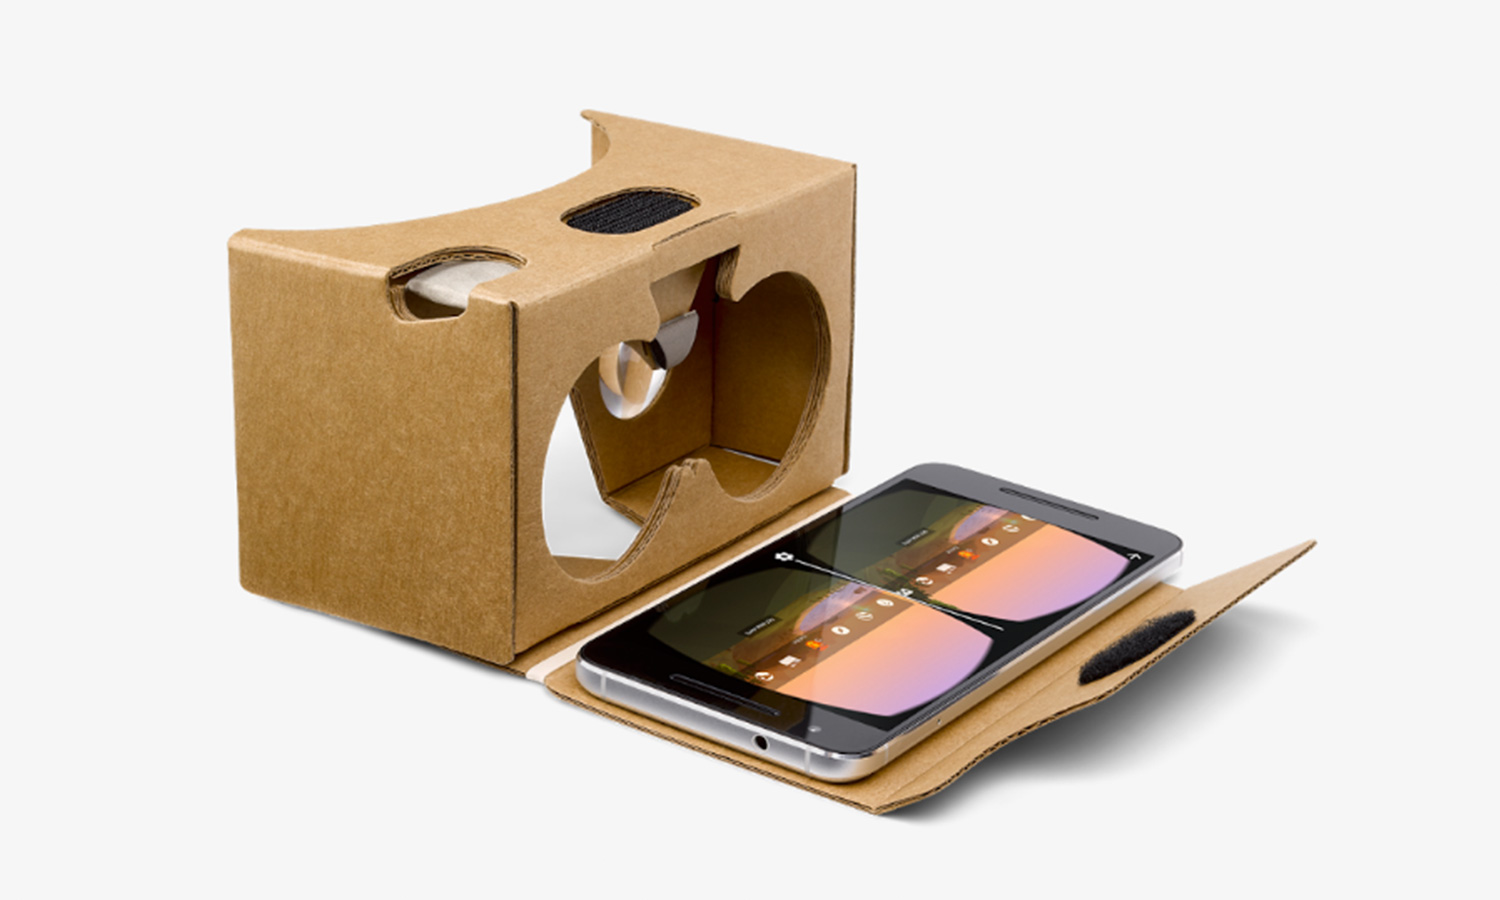
\includegraphics[width=0.75\textwidth]{Images/google_cardboard.jpg}
\end{figure}	

\subsection{Oculus Quest}
The second VR device we looked at was the Oculus Quest. The Oculus Quest is an all in one VR headset that runs a modified version of the Android operating system (OS) \cite{13685558020190801}. It is built using Android 7.1 (Nougat) but can support as far back as Android 4.4 (KitKat). This device is considerably more expensive than the Google Cardboard retailing at 599 EUR for the 128GB model but serves several distinct advantages which are listed below \cite{13685558020190801}.

\begin{figure}[h!]
	\caption{Oculus Quest VR HMD.}
	\label{image:oculusquest}
	\centering
	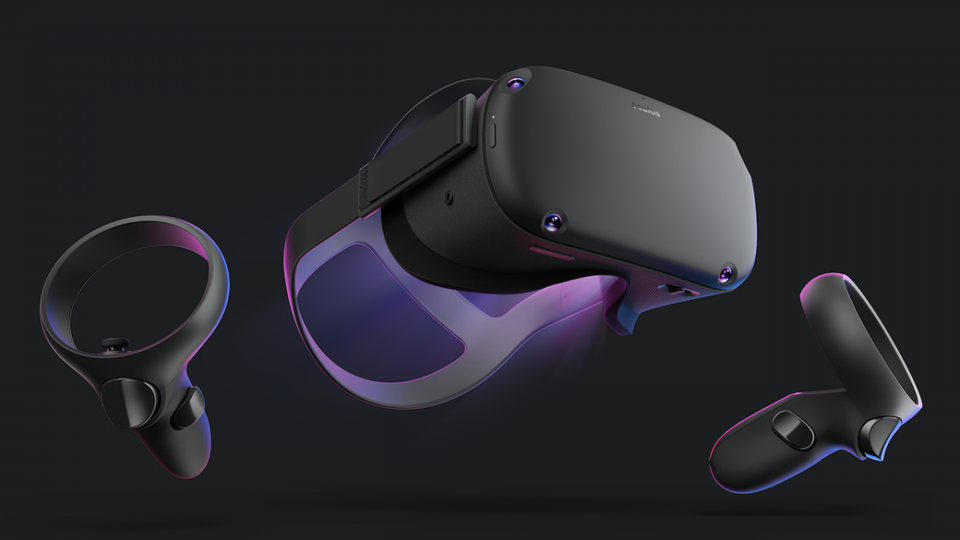
\includegraphics[width=0.75\textwidth]{Images/oculus_quest.png}
\end{figure}

\begin{itemize}
    \item Two 1440 x 1600-pixel screens with a refresh rate of 72 Hz, which provides a clearer and more realistic viewing experience.
    \item Runs on Android so previous builds for Google Cardboard work.
    \item Touch controller support as seen in figure~\ref{image:oculusquest}, so the player can see their hands in the virtual environment and move the player.
    \item Unity support for Oculus Quest.
    \item More comfortable to wear for longer periods of time due to dedicated strap, which is also shown in figure~\ref{image:oculusquest}.
\end{itemize}

\section{Speech Services}
As the application needed to include a dynamic chatbot we looked at some Text-to-Speech (TTS) and Speech-to-Text (STT) services to achieve this. Our initial thought was to include a text input system or a multiple choice dialog tree but from testing and further research we felt it would be pre-programmed and substantially less interactive for a training environment. This spurred us to look at other areas and the possibility of taking in audio from the microphone and parsing it to text using TTS. TTS involves converting human speech to a text format so it can be read by a machine in real time \cite{EJ122858920190101}. On the other hand, STT is the opposite in which text is converted to human like synthesized speech, which would be used to give our chatbot life, personality and evoke possible emotions \cite{ED60067020190801}. Below we will look at some of the technologies we reviewed and tested in these two areas.

\subsection{Windows}
All Windows devices have STT functionality built into its Cortana virtual assistant. This allows the user to talk directly to the device and it will pick up what you said and decide from this. As described above we decided to use Unity as the main technology for our application which would be deployed to and Oculus Quest, so any service we tested must work with Unity and Android respectively. As the Windows STT services provided a Unity package, we thought it could work well, however from testing it was quite slow at depicting speech despite being accurate \cite{unityspeech}. Also, the text predicted was lower case and contained no punctuation, or any useful characters such as question marks etc. which would be useful for determining context in Natural Language processing. Another unfortunate downside was that it didn't work on Android when testing so we decided to look at other options, this was since it's developed for Windows. 

\subsection{Google Cloud}
The second speech service we looked at was Google Cloud Speech Synthesis. Compared to the inbuilt system provided by Windows this service works using an application programming interface (API) where audio data is sent to a remote server and a result is returned \cite{googlespeech}. Because of this a constant internet connection is required which is another issue to look at. Using the documentation provided a solution was implemented despite it not working as desired due to the fact there is no specific Unity package available. The only way to implement it is to add the DLL files in Unity as a source which worked but unfortunately not as desired. Another area where Google Cloud was quite beneficial was the fact that allowed the developer to tailor the Speech Services to their own need. Some options included the ability to change the voice of the response from TTS or changing the pitch and tone of the voice \cite{googlespeech}. This would be useful for depicting emotion in characters. The cost to use Google's services was also quite reasonable and provided a good allowance of free usage which would suffice for our needs but as it didn't work as expected we decided to test other services. 

\subsection{IBM Watson}
Another service we researched was IBM Watson speech services, but with only a very limited amount of free characters (10,000) available for TTS and 250 minutes free with STT we found it to be a costly service to use \cite{ibmspeech}. Another downside again to this service was the fact that there was no Unity package available either, so ultimately, we decided to look into other service providers.

\subsection{Azure}
Much like Google Cloud services Azure works in much the same way and provides the same features regarding multiple voices, tone, pitch etc. which would allow a realistic experience. There is also over 140 different voices provided with 9 specific Neural voices built using machine learning that are specifically designed to provide a realistic human like response. Also, there is support for over 45 languages which could be used for future research to make the application available in multiple countries \cite{azurespeech}. Other benefits include the fact there is a Unity package available for both TTS and STT, along with Android, IOS and Windows support. Another feature which improves on the inbuilt Windows STT is the service can depict punctuation and other useful characters such as question marks etc. which would be useful for Natural Language processing (NLP). Below we will look a more in-dept look at the costs for each service in relation to virtual training.

\subsubsection{Costs - Azure Text-to-Speech}
There would be 250-400 replies an hour on average, with around 12500-20000 characters used per hour (average sentence around 50 characters). Based on the above the free tier would allow up to 25 hours of training for free per month \cite{azurespeechprice}. Additional characters can be purchased for 14 EUR (1 million characters) which would allow for an additional 50 hours of training.

\subsubsection{Costs - Azure Speech-to-Text}
Every reply is on average 3-10 seconds. In one hour of training, it will use around 30 minutes. Based on the above the free tier would allow for up to 10 hours of training for free per month (5 hours free) \cite{azurespeechprice}. A further hour can be purchased for 0.80 EUR, which equates to 2 hours of training. So, an additional 10 hours of training would cost 4.00 EUR.
\newline\newline
From testing, research and analysis of the benefits we decided to use Microsoft Azure services for our application for the following reasons.

\begin{itemize}
  \item Azure provided the best training cost, which would be useful for our client.
  \item Azure provided the most useful custom options in regard to multiple voices, language, pitch tone etc. which would required to scale the project in the future.
  \item Azure STT works extremely well at depicting human speech and includes punctuation. It is also very efficient and accurate.
  \item A Unity package is provided which would allow it to be easily deployed to a Unity environment and run efficiently.
  \item Android and IOS are supported which would allow the service to work on the multiple VR devices reviewed such as the Oculus Quest and Google VR.
\end{itemize}

\section{Chatbot}
It was a given that a we needed to create a chat-bot so this was one of the first areas we started to research. We looked at all the chat-bots created in the past and they all followed a trend. This trend was that they either used machine learning or AIML also known as Artificial Intelligence Markup Language. Before deciding on one from the beginning we tested both technologies to see which was suited best to our requirements. All we needed the bot to do at the start was take in an input and return an accurate and relevant response. Before implementing Speech-to-Text and Text-to-Speech we worked with the most simple form of conveying dialog which was strings of text. We got this working with both the AIML and machine learning approach. Below are the two technologies in more detail and why when chose AIML for our final implementation.

\subsection{Keras}
Keras is a deep learning library that allows you to create neural networks quickly with very little implementation\cite{chollet2018keras}. It also has a dedicated library for python which would run seamlessly on our flask server meaning we could make requests to the neural network using HTTP. To train the model, we processed a JSON intents file that included objects that looked like this:\cite{18Python81:online}

\begin{lstlisting}[language=JSON]
{"intents": [
    {"tag": "greeting",
     "patterns": ["Hi.", "Is anyone there?", "Hello.", "Good day"
        , "Whats up?"],
     "responses": ["Hello!", "Good to see you again!", "Hi there
        , how can I help?"],
     "context_set": ""
    },
    {"tag": "greetingResponse",
      "patterns": ["I am great thanks!", "Great, thank you!"
        , "Not too bad!"],
      "responses": ["That's good to hear.", "I'm glad."],
      "context_set": ""
     }
    ]
}
\end{lstlisting}

The pre-processing mapped certain words to the tag. For example in the above snippet you can see the tag "greeting", and one of the patterns is "Is anyone there?". What the pre-processing does is it creates a bag for words related to the tag removing any unnecessary words like "Is" in this case. Then it trains the model using this tag and that bag of words. It also has a list of responses that is added to the output of the neural network. After training the model keras loaded it and it was ready for use. Pre-processing would have to be done for every input too. This was done using the the method of creating a bag for words. Then that bag of words was used as an input to predict an output/response. The neural network was very accurate however it had some issues:

\begin{itemize}
  \item The model would have to be rebuilt every time more responses where appended to the intents file making it tedious and bulky to maintain.
  \item There was no simple way for creating independent sessions for each bot. This was a feature that we really needed as we knew the application would have many different instances of the bot and that progress/state needed to be saved and there was no simple way of doing it.
\end{itemize}

Initially the we thought the safest approach in creating a chat-bot would be to use a neural network however, after doing some testing and implementing a working build using keras we found out that it was not the right route to take.

\subsection{AIML}
%
Artificial Intelligence Markup Language (AIML) is markup language that allows you to create a set of conversation rules\cite{AIChatBo91:online}. These rules contain various tags and symbols that allow you to generate outputs or responses based on the input. AIML's tags are similar to another markup language called Extensible Markup Language(XML). The reason these markup languages are so similar is due to the fact that AIML is derived from XML. The main reason we chose AIML over the Keras approach was for the simple reason that we needed to store session data. This would have been very difficult to do using keras and would have forced us to do a lot of string manipulation to try and extract the relevant data from the input. AIML had built in tags and methods that allowed us to save various bits of data that we could store on a session by session basis. This was essential to the project and that is why we fundamentally chose AIML over Keras.
\newline

Below is a table of the tags that are most used in AIML and a description of what they do:\cite{aimltuto63:online}\cite{wallace2003elements}
\newline
\begin{tabular}{ |p{3cm}|p{10cm}|  }
\hline
\multicolumn{2}{|c|}{AIML TAGS} \\
\hline
Tag & Description \\
\hline
$<$ aiml $>$ & Defines the beginning and end of a AIML document. \\
\hline
$<$ category $>$ & Defines the unit of knowledge in a bot's knowledge base. \\
\hline
$<$ pattern $>$ & Defines the pattern to match what a user may input to a bot. \\
\hline
$<$ template $>$ & Defines the response of a bot to user's input. \\
\hline
$<$ star $>$ & Used to match wild card * character(s) in the $<$pattern$>$ Tag. \\
\hline
$<$ srai $>$ & Multipurpose tag, used to call/match the other categories. \\
\hline
$<$ random $>$ & Used $<$random$>$to get random responses. \\
\hline
$<$ li $>$ & Used to represent multiple responses. \\
\hline
$<$ set $>$ & Used to set value in an AIML variable. \\
\hline
$<$ get $>$ & Used to get value stored in an AIML variable. \\
\hline
$<$ that $>$ & Used in AIML to respond based on the context. \\
\hline
$<$ topic $>$ & Used in AIML to store a context so that later conversation can be done based on
that context. \\
\hline
$<$ think $>$ & Used in AIML to store a variable without notifying the user. \\
\hline
$<$ condition $>$ & Similar to switch statements in programming language. It helps the bot to respond
to matching input.\\
\hline
\end{tabular}
\newline
\newline

Below is a snippet of the simplest input and output that can be made in AIML. When the user says "HELLO BOT", AIML looks for patterns that contain this string. If the pattern is found, the bot replies with the contents of the template tags which is "Hello User!". However, if the input is not found in the patterns, you can have a category that acts as a catch all using the "*" symbol which will become the default response if no other input was found which in this case would be "Sorry, I do not understand...".

\begin{lstlisting}[language=XML]
<aiml version="1.0.1" encoding="UTF-8"?>
    <category>
    <pattern> HELLO BOT </pattern>
        <template>
            Hello User!
        </template>
    </category>
    
    <category>
    <pattern> * </pattern>
        <template>
            Sorry, I do not understand...
        </template>
    </category>
</aiml>

\end{lstlisting}

With the AIML file set up, all we had to do was access it through our flask server. We were fortunate that python has an AIML library that handles reading the file and saving the state for the chat-bots. Saving the states of every bot was essential for this project and that is why we picked AIML.

\section{Back-end}
To create a fully fledged application we needed a suitable back-end technology to handle the requests from the Unity application over HTTP.

\subsection{Node}
Node.js is an open-source server-side platform that runs and executes using JavaScript. It allows the developer to easily build a fast and scalable network server to run a website, make HTTP requests, etc. \cite{node}. From initial tests we had it running a simple Python file as our chatbot had to be built in Python due to its nature, but that was problematic for Node.js so we investigated other options.

\subsection{Flask}
Flask is a web framework that allows you to build web applications with ease. Flask is actually classed as micro-framework meaning it has very little dependencies to external libraries \cite{flask}. This means Flask is extremely light-weight therefore, very efficient. Because we were working with STT and TTS efficiency was key. We needed to be able to generate responses as quickly as possible to give the illusion that you were having an actual in person conversation with the bot. Flask had this capability along with it being simple to set up so that is why we used it to host the back-end of this application. Below is a snippet of python code to set up a simple working server:

\begin{lstlisting}[language=PYTHON]
from flask import Flask
app = Flask(__name__)

@app.route("/")
def hello():
    return "Hello World!"

if __name__ == "__main__":
    app.run()

\end{lstlisting}

\section{Back-end - Deployment}
After developing and deciding on using Flask as our back-end, we needed to host the server and deploy it in a production build so it could be accessible to devices outside of the local network. A debug server for testing in Flask can only take one request at a time so it's not scalable or secure, so a production build is required. Below is a list of the different options for deploying a Flask server.

\subsection{Self-hosted Options}
Self-hosted solution can be deployed using Web Server Gateway Interface (WSGI) containers. This specification is used to describe how a web service communicates with web applications. A few examples of WSGI containers include Gunicorn, uWSGI, Gevent and Twisted Web \cite{wsgi}. We attempted to implement a WSGI on a Windows Amazon Web Service (AWS) virtual machine (VM) but from research these types of servers are best suited to Linux machines, so we decided to look into other options.

\subsection{Hosted Options - Cloud Services}
There is various platform as a service (PaaS) solutions available to deploy a production server to, which we will look at below. PaaS is a model provided by third party vendors, where the vendor hosts the hardware and software on their own virtual machines and provides access at an affordable cost, which is usually much cheaper than setting up your own machines \cite{heroku}. Below we will review two options that we assessed, tested and used for development.

\subsubsection{Heroku}
Heroku is a PasS which allows developers to build, run and deploy applications easily and efficiently to the cloud \cite{heroku}. Git version control software is used to update, modify and deploy quickly. Heroku also provides a free tier services for student so it is a cost-effective approach to allowing applications to be easily accessible around the world, which is what we required to access our server from an Oculus Quest VR device. There was a few downsides to Heroku though. The first one being an issue with AIML. AIML allows you to store session data/variables which would enable you to save names and other data relevant to each NPC. Heroku had a problem storing this session data making it very difficult to save the states of all the different NPCs/bots in the application so we had to find a different deployment service. Another issue we found was that Heroku would timeout quickly if there was no incoming requests. This made the initial request slow to respond because you would have to wait for Heroku to launch the server.

\subsubsection{PythonAnywhere}
PythonAnywhere is what we decided to use after testing Heroku. It is very similar to Heroku as it allow developers to build, run and deploy their applications on the cloud. However, it differs in a few ways. The free tier of PythonAnywhere allowed the server to stay live for 3 months at a time making initial requests to the flask server much quicker \cite{pythonanywhere}. You could also opt for a paid tier which keeps it live based on a certain amount of usage but the free tier was perfect for testing. Another way that it differs from Heroku is that there is no Git version control instead using an online IDE on their site which allows you to edit all your files from anywhere on any device \cite{pythonanywhere}. Finally the main reason we choose PythonAnywhere, it did not have the issue with saved AIML sessions that Heroku did. This was a deal breaker for us because we needed these sessions for the bots and without them it would have been very difficult to save the states for the bots. 

\section{Databases}
The results of the training simulation needed to be stored somewhere so they could be studied by the testing centre at a later date, so we began to look into possible options to achieve this. For this project we have chosen MongoDB as our database storage technology.

\subsection{MongoDB}
MongoDB is a document oriented distributed database, that allows users to store data quickly, efficiently and securely \cite{mongodb}. The data stored in binary format called BSON, but it is JSON in its human readable form as seen below.

\begin{lstlisting}[language=JSON]
{
  "_id": "5cf0029caff5056591b0ce7d",
  "firstname": "Jane",
  "lastname": "Wu",
  "address": {
    "street": "1 Circle Rd",
    "city": "Los Angeles",
    "state": "CA",
    "zip": "90404"
  },
  "hobbies": ["surfing", "coding"]
}
\end{lstlisting}

\subsubsection{Advantages}
\begin{itemize}
    \item High speed - MongoDB is a document-orientated database. It is easy to access documents by indexing. Hence, it provides a fast query response. It is estimated to be 100 times faster than a relational database.
    \item Sharding - Allows storage of large pieces of data by distributing to several servers, this also improves read times.
    \item Flexible - MongoDB is a schema-less database. That means we can have any type of data in a separate document. This allows us to store data of different types.
    \item Easy environment setup - Easier to setup than a relational database. Also provides Flask plugin called PyMongo which allows easy connection to the database.
\end{itemize}

\subsection{mLab}
mLab is a Database-as-a-Service (DAAS) for MongoDB, it is a free to use provider that allows for cloud hosting for your MongoDB database \cite{mlab}. We have decided to use this technology as we have experience using it and wanted to learn more. There are also useful Flask plugins provided which allow a connection easily to mLab.

\section{Other areas of research}
As outlined in our introduction the focus of this application was to provide a realistic and gamified training experience that would be useful to the user specifically in the area of conflict resolution. To succeed with this we researched areas such as Digital Twins, Sara de Freitas, Michael J Sutton, Serious Fun, Gamification and Digital Training/VR Training. This research can be found in our "Research" section on GitHub repository.